%\section{Datenvisualisierung}
%
%\frame{
%  \frametitle{Überblick}
%  \tableofcontents[currentsection,hidesubsections,firstsection=35]
%}


\begin{frame}
	\frametitle{Datenvisualisierung}
	
	\epigraph{Es gibt nur eine Breitbandverbindung ins Gehirn.}{\textit{David Kriesel}}
\end{frame}


%\begin{frame}[fragile]
%\frametitle{Datenvisualisierung: Beispiel}
%
%\begin{minted}{python}
%m = df.groupby('release_year').size()
%m.idxmax(), m.loc[m.idxmax()]
%# (2021, 125)
%
%m = df.groupby('date_added').size()
%m.idxmax(), m.loc[m.idxmax()]
%# (Timestamp('2019-11-12 00:00:00'), 722)
%\end{minted}
%\end{frame}


\begin{frame}[fragile]
\frametitle{Datenvisualisierung: Beispiel 1}

\begin{minted}[fontsize=\scriptsize]{python}
m = df.groupby('release_year').size()
m.idxmax(), m.loc[m.idxmax()]
# (2021, 125)

nbins = int(df['release_year'].max() - df['release_year'].min() + 1)
px.histogram(df, x='release_year', nbins=nbins)
\end{minted}

\begin{center}
	\vspace{-\baselineskip}
	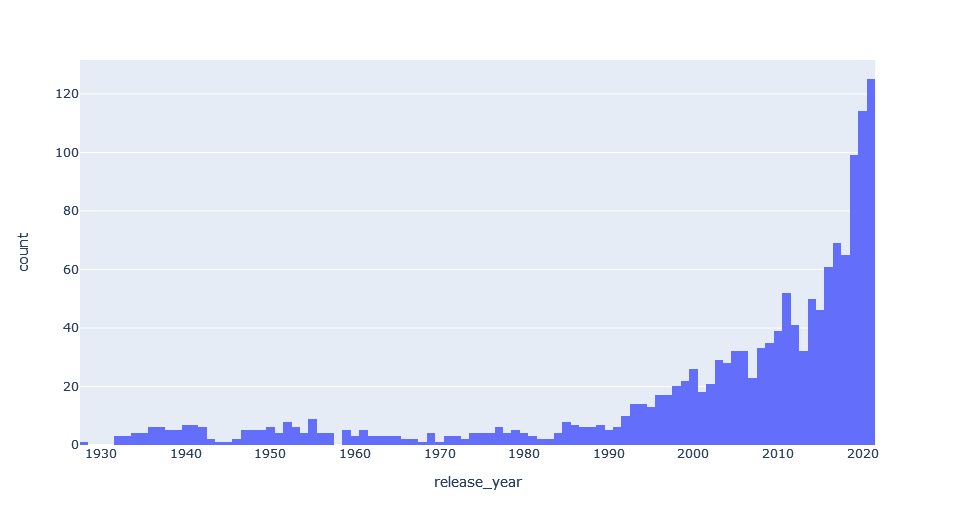
\includegraphics[height=0.5\textheight]{fig5/histogram1.png}
\end{center}
\end{frame}


\begin{frame}[fragile]
\frametitle{Datenvisualisierung: Beispiel 2}

\begin{minted}[fontsize=\scriptsize]{python}
m = df.groupby('date_added').size()
m.idxmax(), m.loc[m.idxmax()]
# (Timestamp('2019-11-12 00:00:00'), 722)

px.histogram(df, x='date_added')
\end{minted}

\begin{center}
	\vspace{-\baselineskip}
	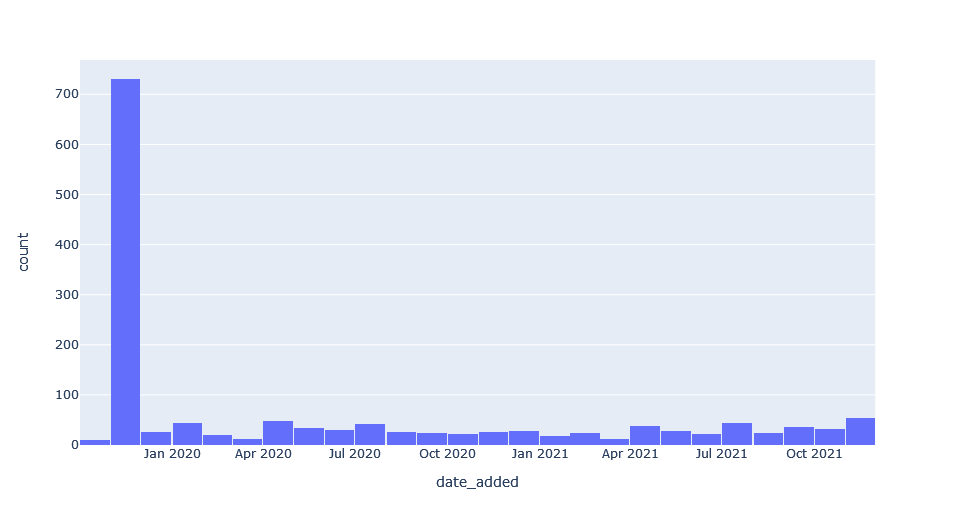
\includegraphics[height=0.5\textheight]{fig5/histogram2.png}
\end{center}
\end{frame}


\begin{frame}[fragile]
\frametitle{Python-Bibliotheken zur Visualisierung}

\begin{itemize}
	\item Matplotlib - Visualization with Python
	\item seaborn: statistical data visualization
	\item \hl{Plotly.py} - Plotly Python Graphing Library
\end{itemize}

\begin{minted}{python}
import plotly.express as px

px.bar(df, x='attr_x', y='attr_y',
       title='Produktionen pro Jahr',
       labels={'attr_x': 'X Werte', 'attr_y': 'Y Werte'})
\end{minted}
\end{frame}


\begin{frame}
\frametitle{Histogramme}

\begin{itemize}
	\item eine Art Säulendiagramm
	\item relative und absolute Häufigkeiten
	\item Klasseneinteilung in sog. \alert{Bins} (Behälter)
\end{itemize}
\end{frame}


\begin{frame}[fragile]
\frametitle{Histogramme}

\begin{minted}{python}
import plotly.express as px
px.histogram(df, x='release_year', nbins=nbins)
\end{minted}

\begin{minipage}{0.5\textwidth}%
\begin{center}%
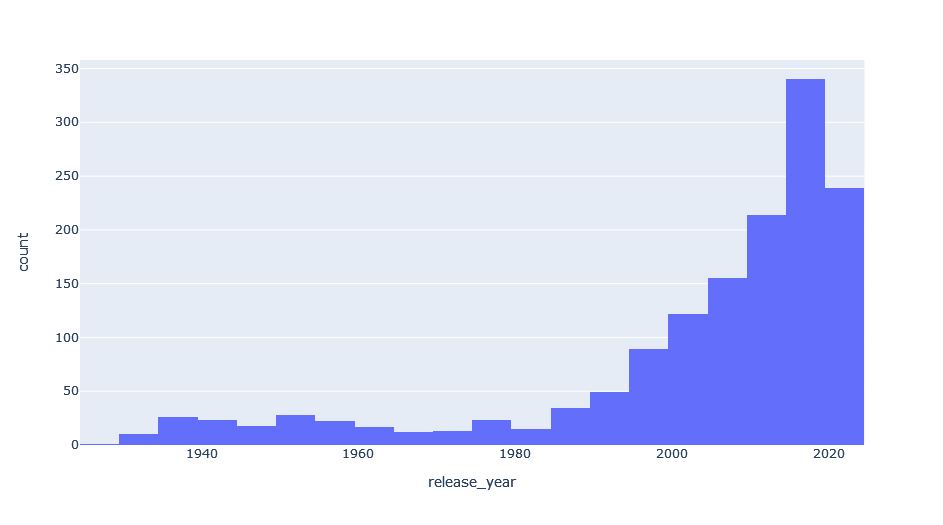
\includegraphics[width=\linewidth]{fig5/histogram3.png}%
\end{center}%
\end{minipage}%
\begin{minipage}{0.5\textwidth}%
\begin{center}%
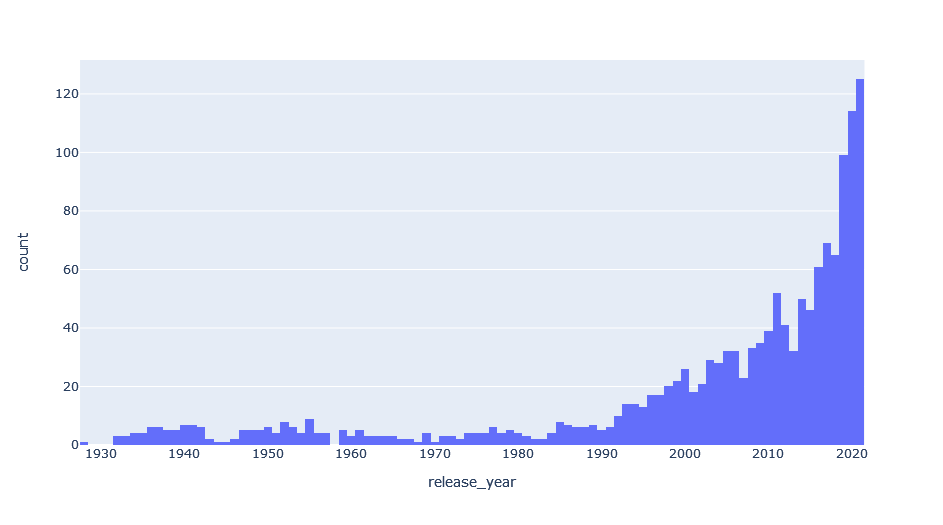
\includegraphics[width=\linewidth]{fig5/histogram4.png}%
\end{center}%
\end{minipage}%
\end{frame}


\begin{frame}
\frametitle{Liniendiagramme}

\begin{itemize}
\item Menge von Punkten durch Linie verbunden
\item suggeriert Kontinuität (stetige Funktionen bevorzugt!)
\end{itemize}
\end{frame}


\begin{frame}[fragile]
\frametitle{Liniendiagramme}

\begin{minted}{python}
import plotly.express as px
px.line(df, x='year', y='total_assets')
\end{minted}

\vspace{-\baselineskip}

\begin{center}
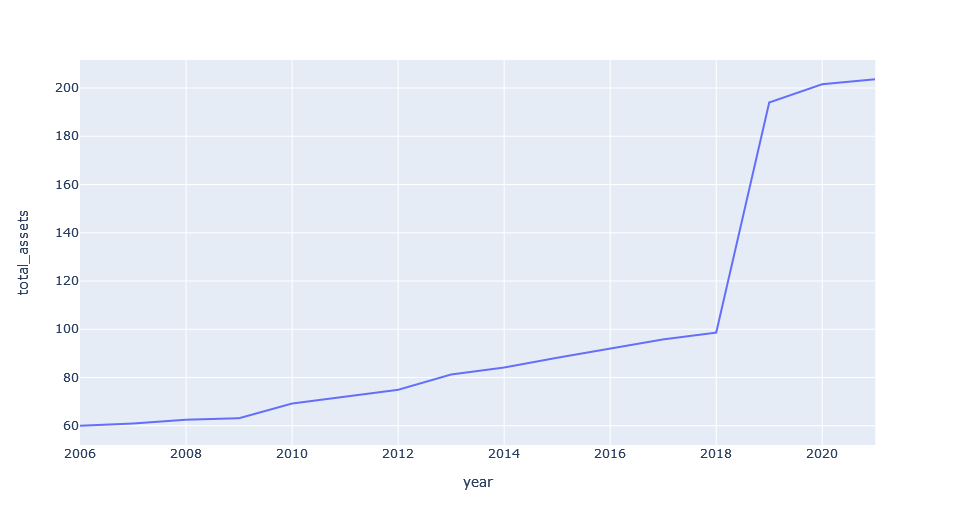
\includegraphics[width=0.85\linewidth]{fig5/line1.png}
\end{center}
\end{frame}


\begin{frame}
\frametitle{Balken- und Säulendiagramme}

\begin{itemize}
\item \textit{vergleichende} Diagramme
\item Höhe der Balken proportional zur Ausprägung des Merkmals
\item in seltenen Fällen auch die Fläche
\end{itemize}
\end{frame}


\begin{frame}[fragile]
\frametitle{Balken- und Säulendiagramme}

\begin{minted}{python}
import plotly.express as px
px.bar(df, x='country', y='movies')
\end{minted}

\vspace{-\baselineskip}

\begin{center}
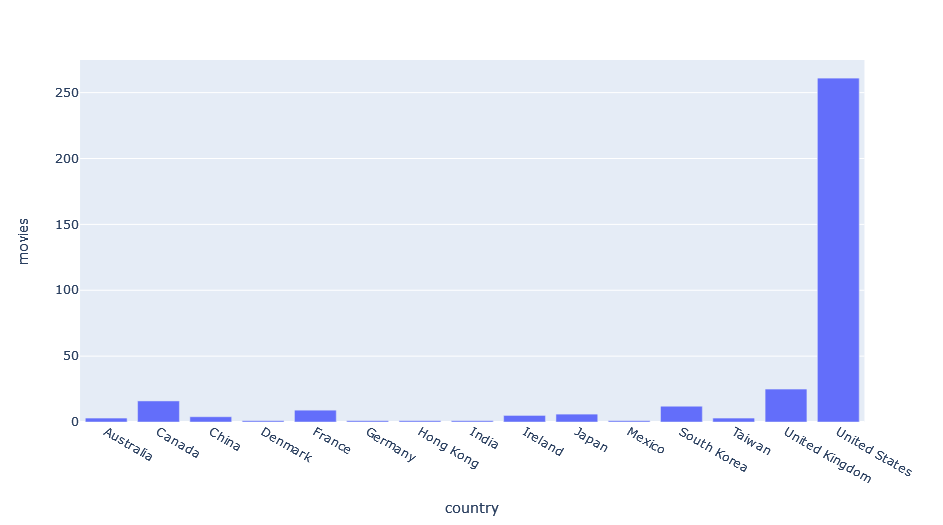
\includegraphics[width=0.85\linewidth]{fig5/bar1.png}
\end{center}
\end{frame}


\begin{frame}[fragile]
\frametitle{Balken- und Säulendiagramme}

\begin{minted}{python}
import plotly.express as px
px.bar(df, x='country', y='movies', orientation='h')
\end{minted}

\vspace{-\baselineskip}

\begin{center}
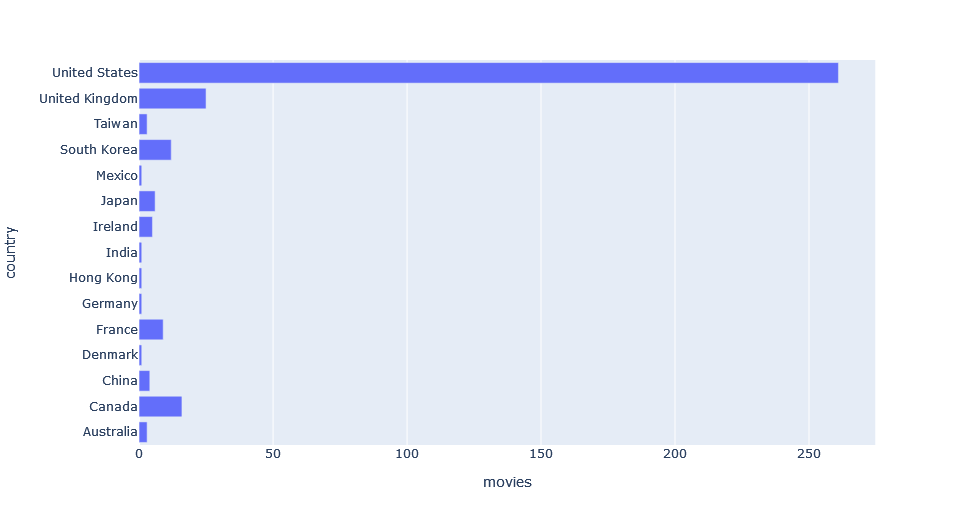
\includegraphics[width=0.85\linewidth]{fig5/bar2.png}
\end{center}
\end{frame}


\begin{frame}[fragile]
\frametitle{Balken- und Säulendiagramme}

\begin{minted}{python}
import plotly.express as px
px.bar(df, x='country', y=['movies', 'tvshows'], log_y=True,
       barmode=...)
\end{minted}

\begin{minipage}{0.5\textwidth}%
\begin{center}%
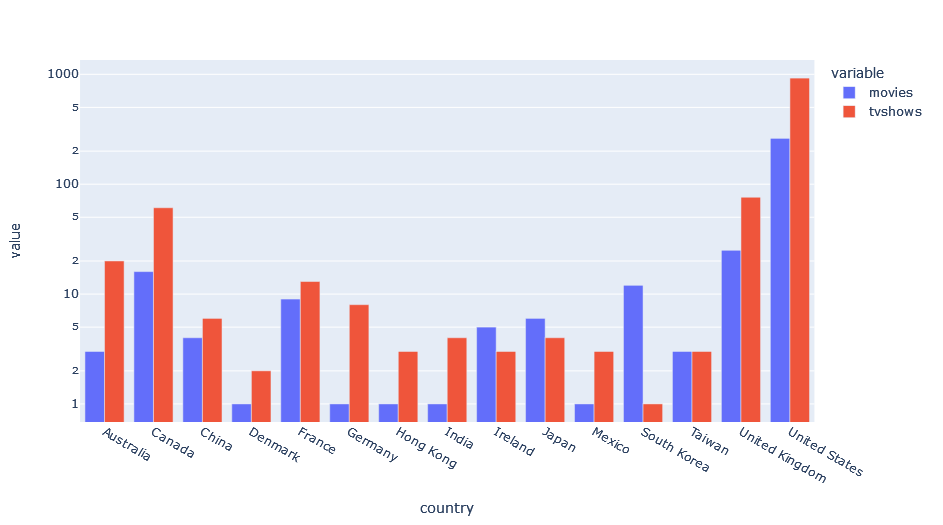
\includegraphics[width=\linewidth]{fig5/bar3.png}%
\end{center}%
\end{minipage}%
\begin{minipage}{0.5\textwidth}%
\begin{center}%
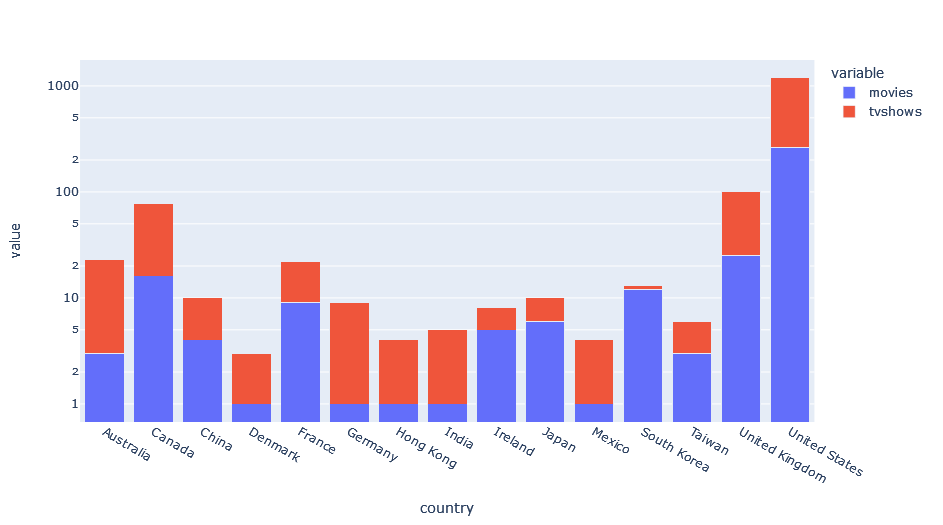
\includegraphics[width=\linewidth]{fig5/bar4.png}%
\end{center}%
\end{minipage}%

\begin{minipage}{0.5\textwidth}%
\begin{center}%
\scriptsize \textit{group}
\end{center}%
\end{minipage}%
\begin{minipage}{0.5\textwidth}%
\begin{center}%
\scriptsize \textit{stack}
\end{center}%
\end{minipage}%
\end{frame}


\begin{frame}[fragile]
\frametitle{Balken- und Säulendiagramme}

\begin{minted}{python}
import plotly.express as px
px.bar(df, x='release_year', y='duration', error_y='sem')
\end{minted}

\vspace{-\baselineskip}

\begin{center}
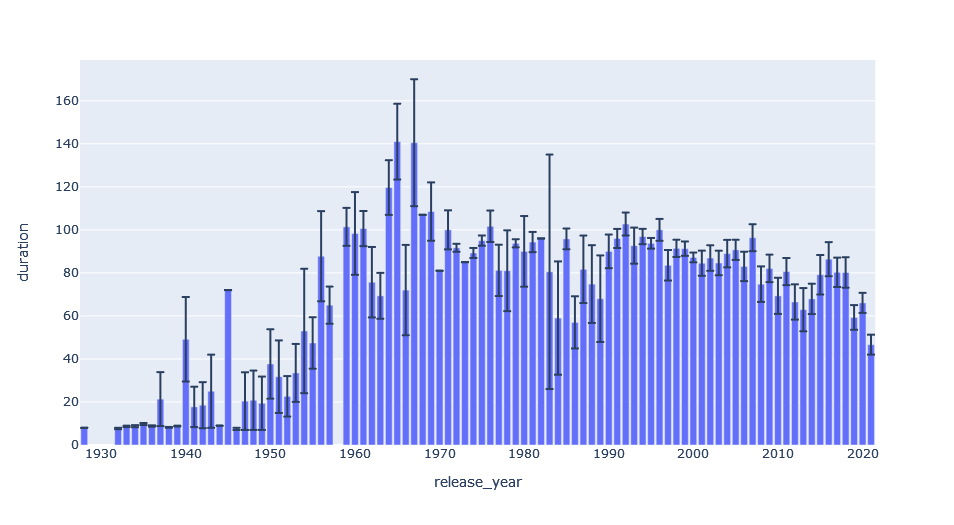
\includegraphics[width=0.85\linewidth]{fig5/bar5.png}
\end{center}
\end{frame}


\begin{frame}
\frametitle{Kreisdiagramme}

\begin{itemize}
\item Darstellung relativer Anteile
\item dreidimensional als Kuchen- oder Tortendiagramm
\end{itemize}

\begin{center}
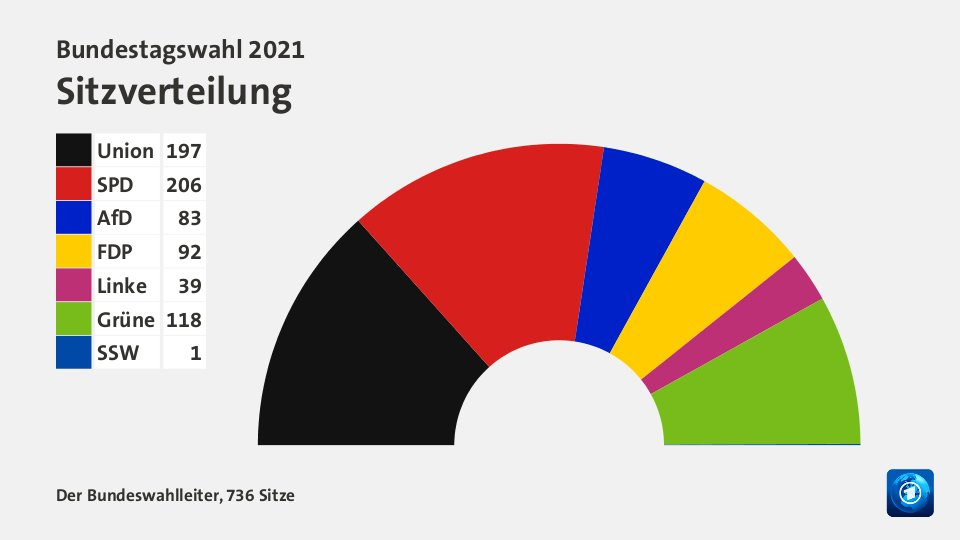
\includegraphics[width=0.85\linewidth]{fig5/pie1.jpg}
\end{center}
\end{frame}


\begin{frame}[fragile]
\frametitle{Kreisdiagramme}

\begin{minted}{python}
import plotly.express as px
px.pie(df, values='count', names='name')
\end{minted}

\vspace{-\baselineskip}

\begin{center}
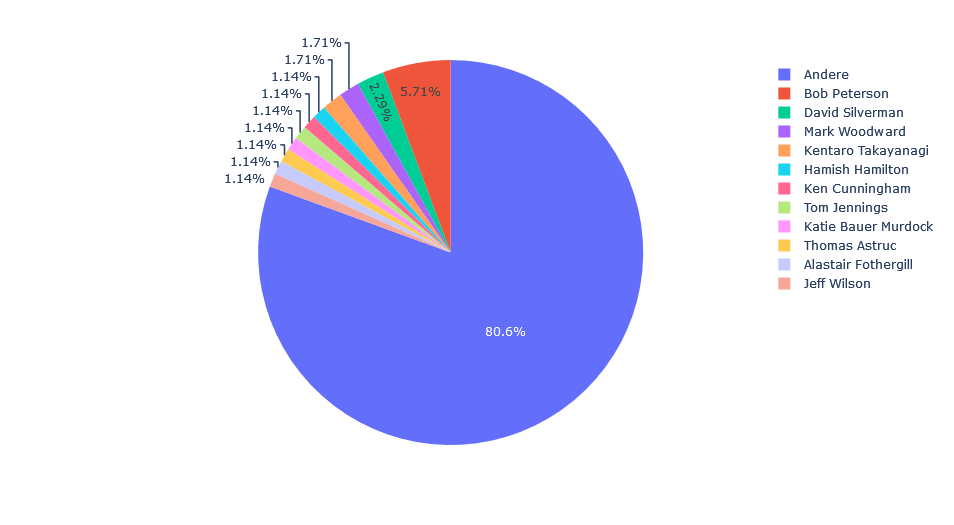
\includegraphics[width=0.85\linewidth]{fig5/pie2.png}
\end{center}
\end{frame}


\begin{frame}[fragile]
\frametitle{Kreisdiagramme}

\begin{minted}{python}
import plotly.express as px
px.pie(df, values='count', names='name',
       hole=0.5)
\end{minted}

\vspace{-\baselineskip}

\begin{center}
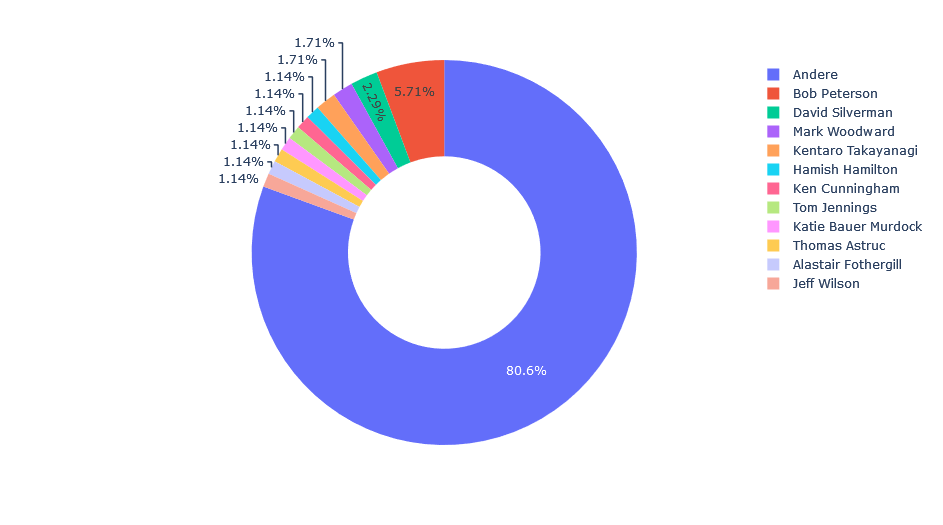
\includegraphics[width=0.85\linewidth]{fig5/pie3.png}
\end{center}
\end{frame}


\begin{frame}[fragile]
\frametitle{Kreisdiagramme}

\begin{minted}{python}
import plotly.express as px
fig = px.pie(df, names='type', values='count')
fig.update_traces(pull=[0.25, 0, 0])
\end{minted}

\vspace{-\baselineskip}

\begin{center}
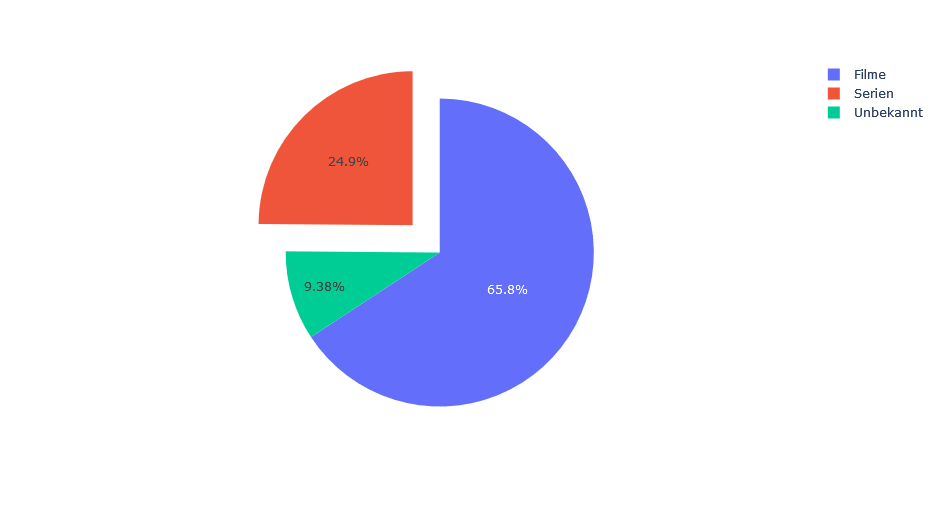
\includegraphics[width=0.80\linewidth]{fig5/pie4.png}
\end{center}
\end{frame}


\begin{frame}
\frametitle{Streudiagramme}

\begin{itemize}
	\item Punktwolke
	\item jedes Wertepaar einzeln
	\item Wiedererkennung statistischer Merkmale
\end{itemize}
\end{frame}


\begin{frame}[fragile]
\frametitle{Streudiagramme}

\begin{minted}{python}
import plotly.express as px
px.scatter(df, x='release_year', y='duration_in_minutes')
\end{minted}

\vspace{-\baselineskip}

\begin{center}
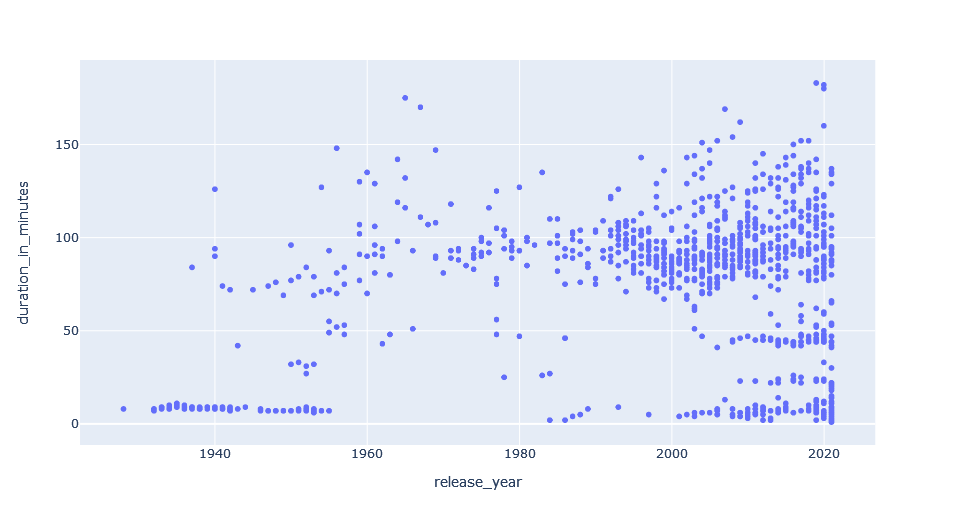
\includegraphics[width=0.80\linewidth]{fig5/scatter1.png}
\end{center}
\end{frame}


\begin{frame}[fragile]
\frametitle{Streudiagramme}

\begin{minted}{python}
import plotly.express as px
px.scatter(df, x='release_year', y='duration_in_minutes',
           size='cast_size')
\end{minted}

\vspace{-\baselineskip}

\begin{center}
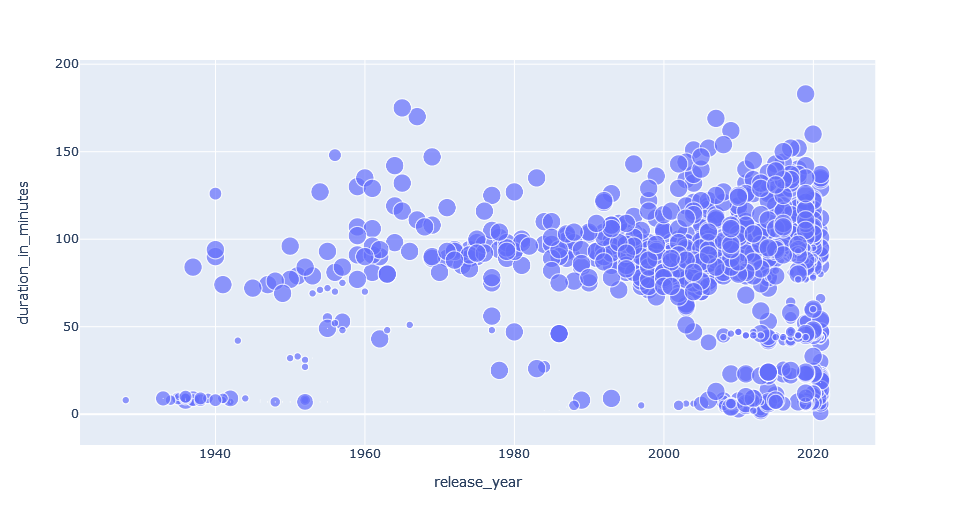
\includegraphics[width=0.80\linewidth]{fig5/scatter2.png}
\end{center}
\end{frame}


\begin{frame}[fragile]
\frametitle{Streudiagramme}

\begin{minted}{python}
import plotly.express as px
px.scatter(df, x='release_year', y='duration_in_minutes',
           color='cast_size')
\end{minted}

\vspace{-\baselineskip}

\begin{center}
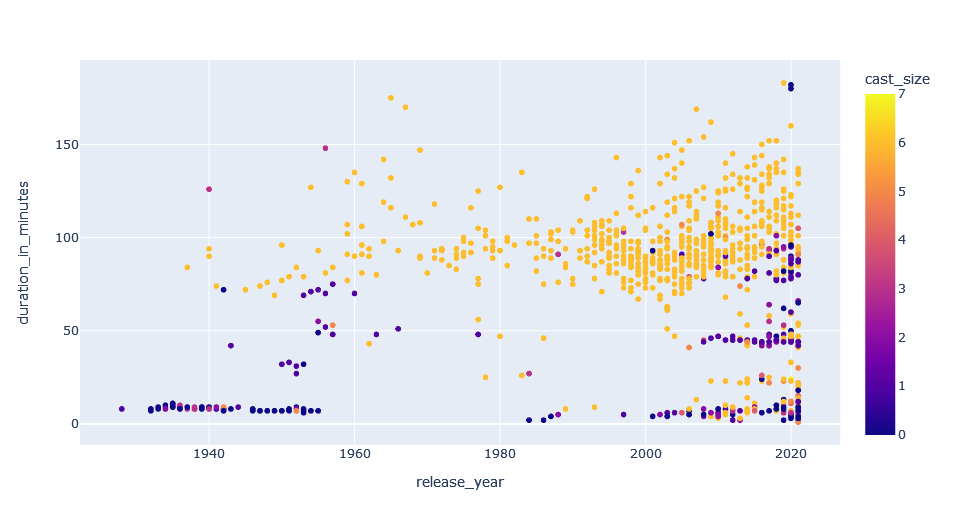
\includegraphics[width=0.80\linewidth]{fig5/scatter3.png}
\end{center}
\end{frame}


\begin{frame}[fragile]
\frametitle{Streudiagramme}

\begin{minted}{python}
import plotly.express as px
px.scatter(df, x='release_year', y='duration_in_minutes',
           symbol='director_size')
\end{minted}

\vspace{-\baselineskip}

\begin{center}
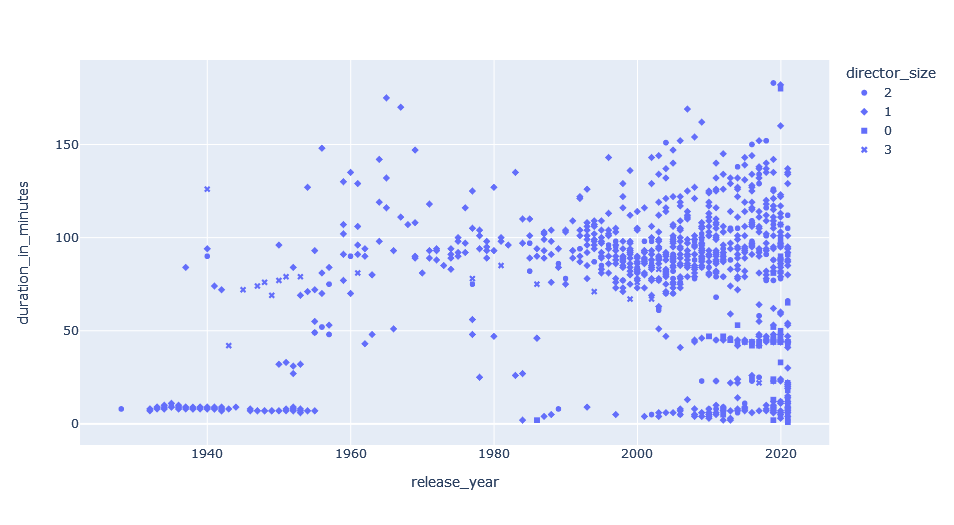
\includegraphics[width=0.80\linewidth]{fig5/scatter4.png}
\end{center}
\end{frame}


\begin{frame}
\frametitle{Streudiagramm-Matrix}

\begin{itemize}
	\item paarweise Streudiagramme
	\item Aufdecken statistischer Zusammenhänge
\end{itemize}
\end{frame}


\begin{frame}[fragile]
\frametitle{Streudiagramm-Matrix}

\begin{minted}{python}
import plotly.express as px
px.scatter_matrix(df[['date_added', 'release_year', 'rating', 'duration']])
\end{minted}

\vspace{-\baselineskip}

\begin{center}
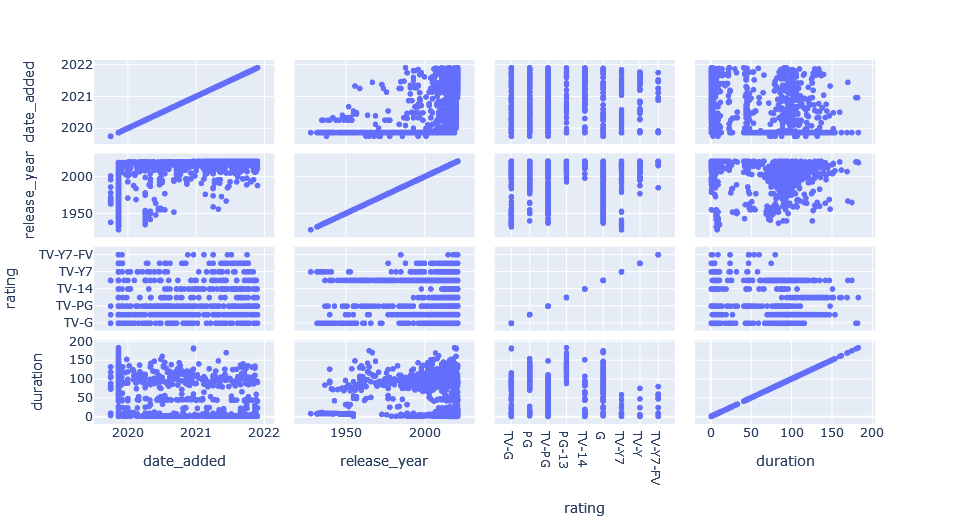
\includegraphics[width=0.80\linewidth]{fig5/matrix1.png}
\end{center}
\end{frame}


\begin{frame}
\frametitle{Streudiagramm-Matrix}

\begin{center}
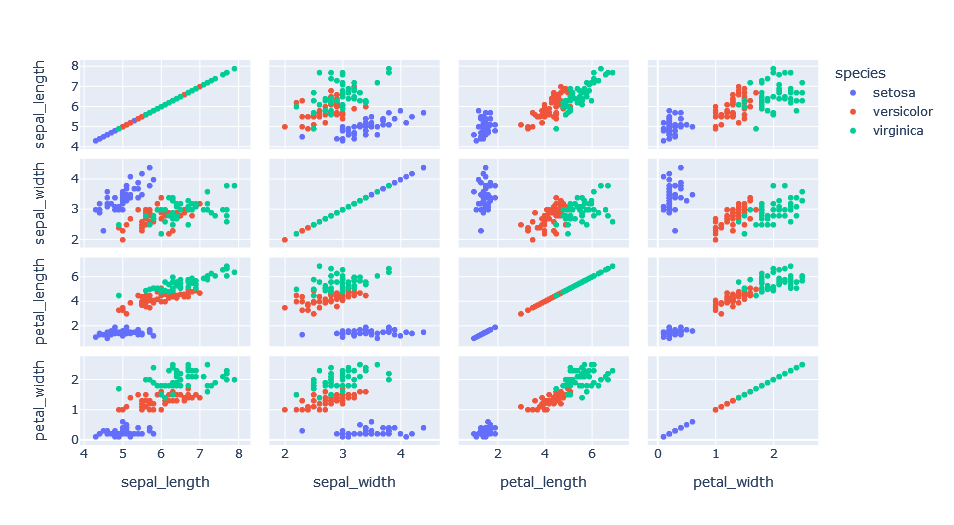
\includegraphics[width=\linewidth]{fig5/matrix2.png}
\end{center}
\end{frame}
